\section{Our Construction}\label{sec:construction}



\subsection{Overview}

Our core protocol is a technique for obliviously mapping together records that have keys with the same value. In particular, for each secret shared row $\share{X}[i]$ our protocol obliviously maps rows $\share{Y[j_0]},\share{Y[j_1]}$ to the $i$th position of two new tables $\share{Y'_0},\share{Y'_1}$ such that if there exists a matching key in $Y$ then $\share{Y'_0}[i]$ or $\share{Y'_1}[i]$ will contain this row. In the event that no such key exists in $Y$ then arbitrary rows from $Y$ are mapped to these locations instead. Once the mapping is performed the output table can be constructed by an MPC protocol\cite{aby3} that directly compares the keys for the $i$th row of $\share X$ and $\share{Y'_0},\share{Y'_1}$. 

Without loss of generality let us assume that the columns $X_0$ and $Y_0$ are the keys being joined on. Our protocol begins by generating a \emph{randomized encoding} for each of the secret shared elements $\share x\in \share{X_0}$ and $ \share y\in \share{Y_0}$. \figureref{fig:randomized-encode-ideal} contains the ideal functionality for this encoding which take secret shares from the parties, apply a PRF $F_k$ to the reconstructed value using a internally sampled key $k$, and returns the resulting value to one of the three parties. For $\share x\in \share{X_0}$, party 0 will learn $F_k(x)$ while party 1 will learn $F_k(y)$ for $\share y\in \share{Y_0}$.

Party 1 proceeds by constructing a \emph{secret shared} cuckoo hash table $\share{\hat Y}$ for the rows of $\share{Y}$ where the hash function values employed are defined as $h_i(y) = H( i || F_k(y))$. That is, party 1 knows the hash function values but the contents of the hash table remains secret shared between the parties. To prevent the parties 0 and 2 from learning information about the randomized encodings $F_k(y)$, party 1 must obliviously permute their shares to the desired position of the cuckoo hash table. We achieve this using a three party oblivious permutation protocol which further randomizes the secret shares to prevent leakage.

It is now the case that $\share{\hat Y}$ is a valid cuckoo hash table of $\share Y$ which is in a secret shared format. Party 0, who knows the randomized encodings $F_k(x)$ for all $\share x\in \share{X_0}$, now must query $\share{\hat Y}$ at the slots indexed by $h_i(x)= H( i || F_k(x))$ and compare this with the corresponding row of $\share X$. In particular, assuming we use two cuckoo hash functions, then party 0 constructs two \emph{oblivious switching networks} that maps the shares $\share{\hat Y[{h_0(x)}]}$ and $\share{\hat Y[{h_1(x)}]}$ to be aligned with $\share x$.

Once the shares  $\share{\hat Y[{h_0(x)}]}, \share{\hat Y[{h_1(x)}]}$ and $\share x$ are aligned, the parties employ an MPC protocol to directly compare the joined on columns/keys to compute a secret shared bit denoting whether $x$ matches with one of the rows. When computing an inner join query, only rows of $X$ where the comparison bit is set to one are considered valid while the other rows are set to \texttt{NULL}. Note that when columns of $Y$ are selected the corresponding values are obtained from $\share{\hat Y[{h_i(x)}]}$ for the $i$ that the comparison succeeded on. Left joins work in a similar way except that all rows of $X$ are included while the comparison bit is used to select the columns of $Y$ or set the fields to \texttt{NULL}. Finally, unions can be computed by including all of $Y$ in the output and all of the rows of $X$ where the comparison bit is set to zero. Regardless of the type of join, the protocols do not reveal any information about the tables. In particular, not even the cardinality of the join is revealed.

\iffullversion
\begin{figure}\centering
	\frame{	\begin{tikzpicture}[scale=0.6, every node/.style={scale=0.6}]
	\draw (0, 0) node[inner sep=0] {{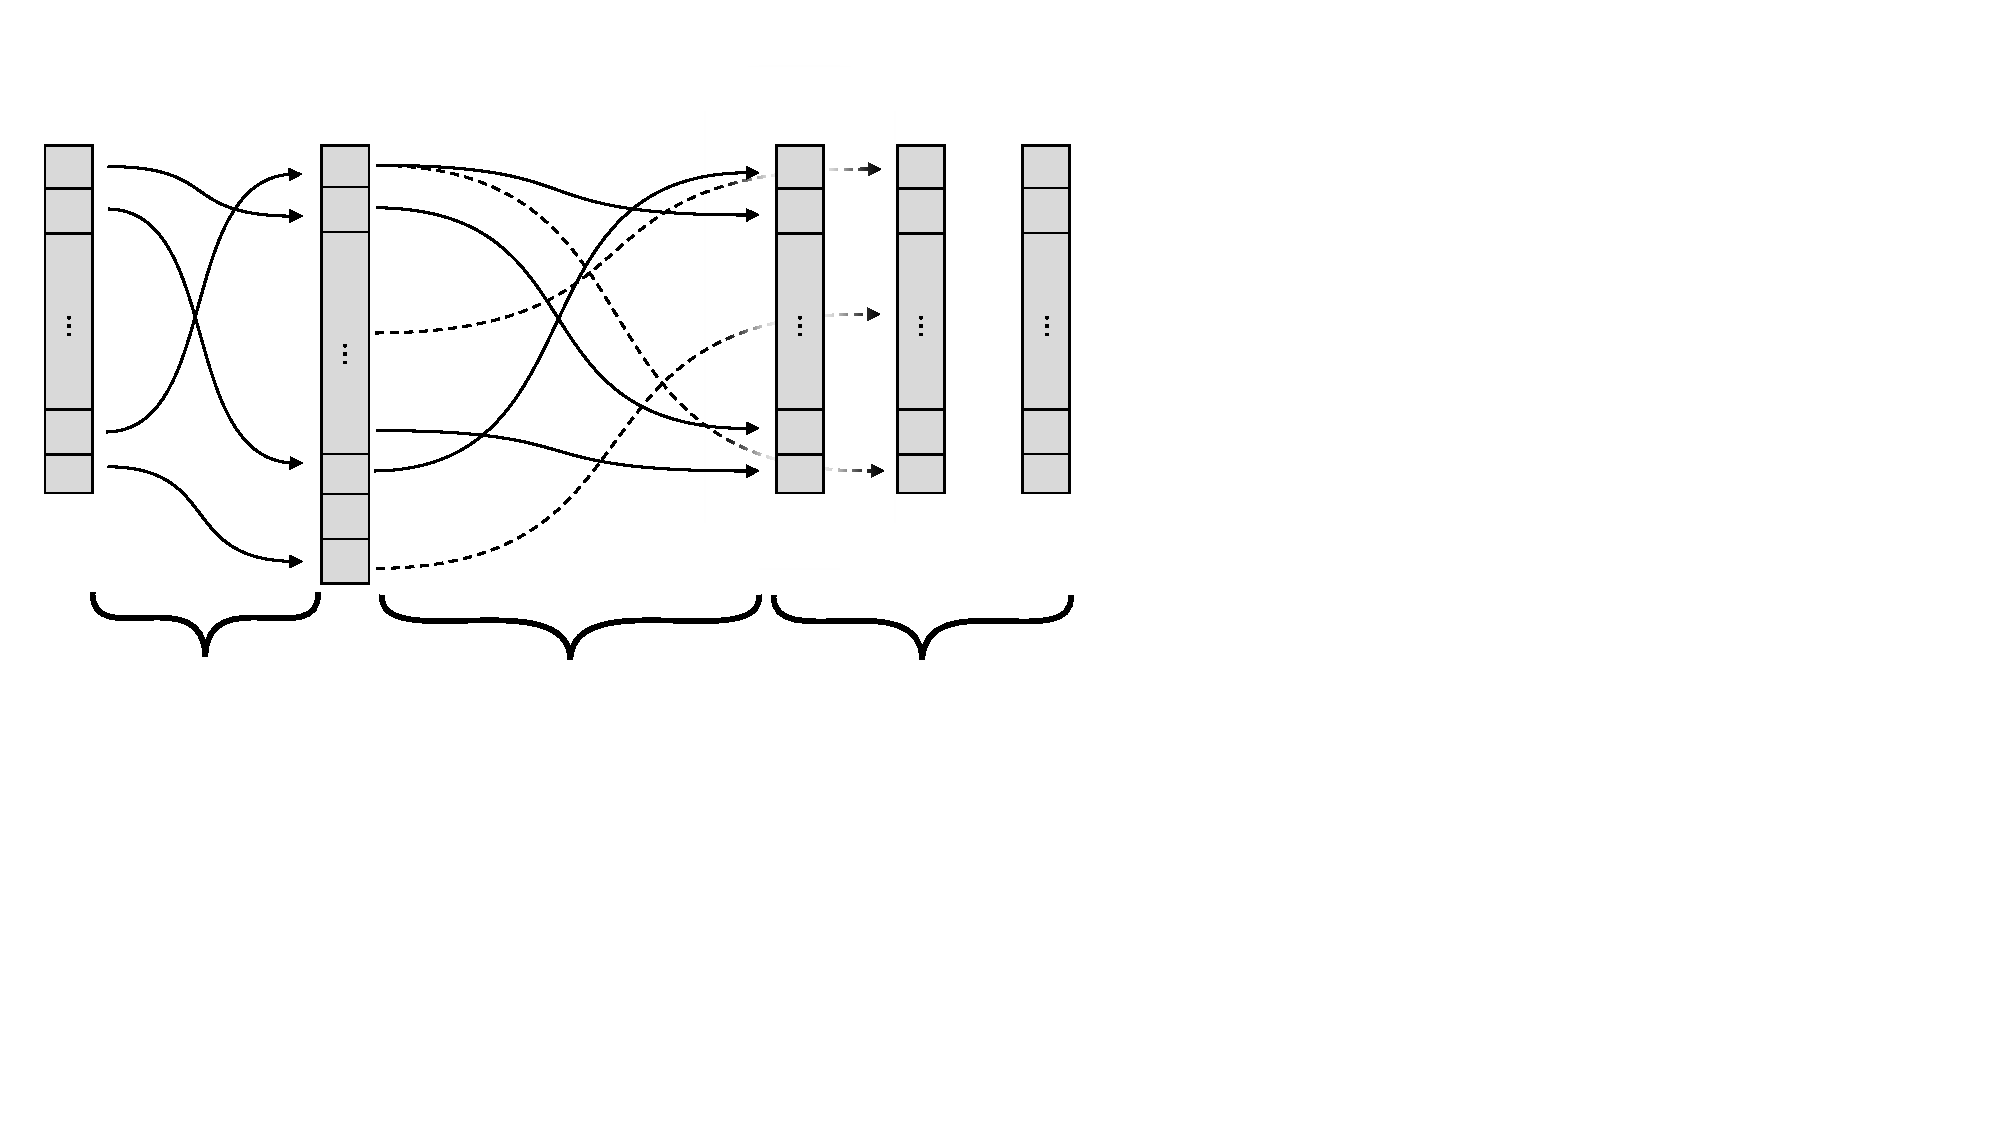
\includegraphics[trim={0cm 7cm 14cm 1cm},clip,width=\textwidth]{diga.pdf}}};
	\draw (-7.3cm,4cm) node {\large$Y$};
	\draw (6.5cm,4cm) node {\large$X$};
	\draw (-3.3cm,4cm) node {\large$\hat Y$};
%	\draw (3.8cm,4.6cm) node {\large Selections w/ $h_0(x),h_1(x)$};
	\draw (3cm,4cm) node { \large$Y'_0$};
	\draw (4.7cm,4cm) node { \large$Y'_1$};
	
	\draw (-5.2cm,-4.1cm) node { Cuckoo hash w/ };
	\draw (-5.2cm,-4.6cm) node { $\textsc{encode}(Y)$ \& oblv. };
	\draw (-5.2cm,-5.1cm) node { permutation};
	
	
	\draw (0cm,-4.1cm) node { Select Cuckoo locations w/ };
	\draw (0cm,-4.6cm) node {  $\textsc{encode}(X)$ \& Oblv.};
	\draw (0cm,-5.1cm) node { switching net.};
	
	
	
	\draw (5cm,-4.1cm) node { Compare w/ circuit };
	\end{tikzpicture}}
	\caption{Overview of the join protocol using oblivious switching network.}
\end{figure}
\else
\begin{figure}\centering
	\frame{	\begin{tikzpicture}[scale=0.48, every node/.style={scale=0.48}]
		\draw (0, 0) node[inner sep=0] {{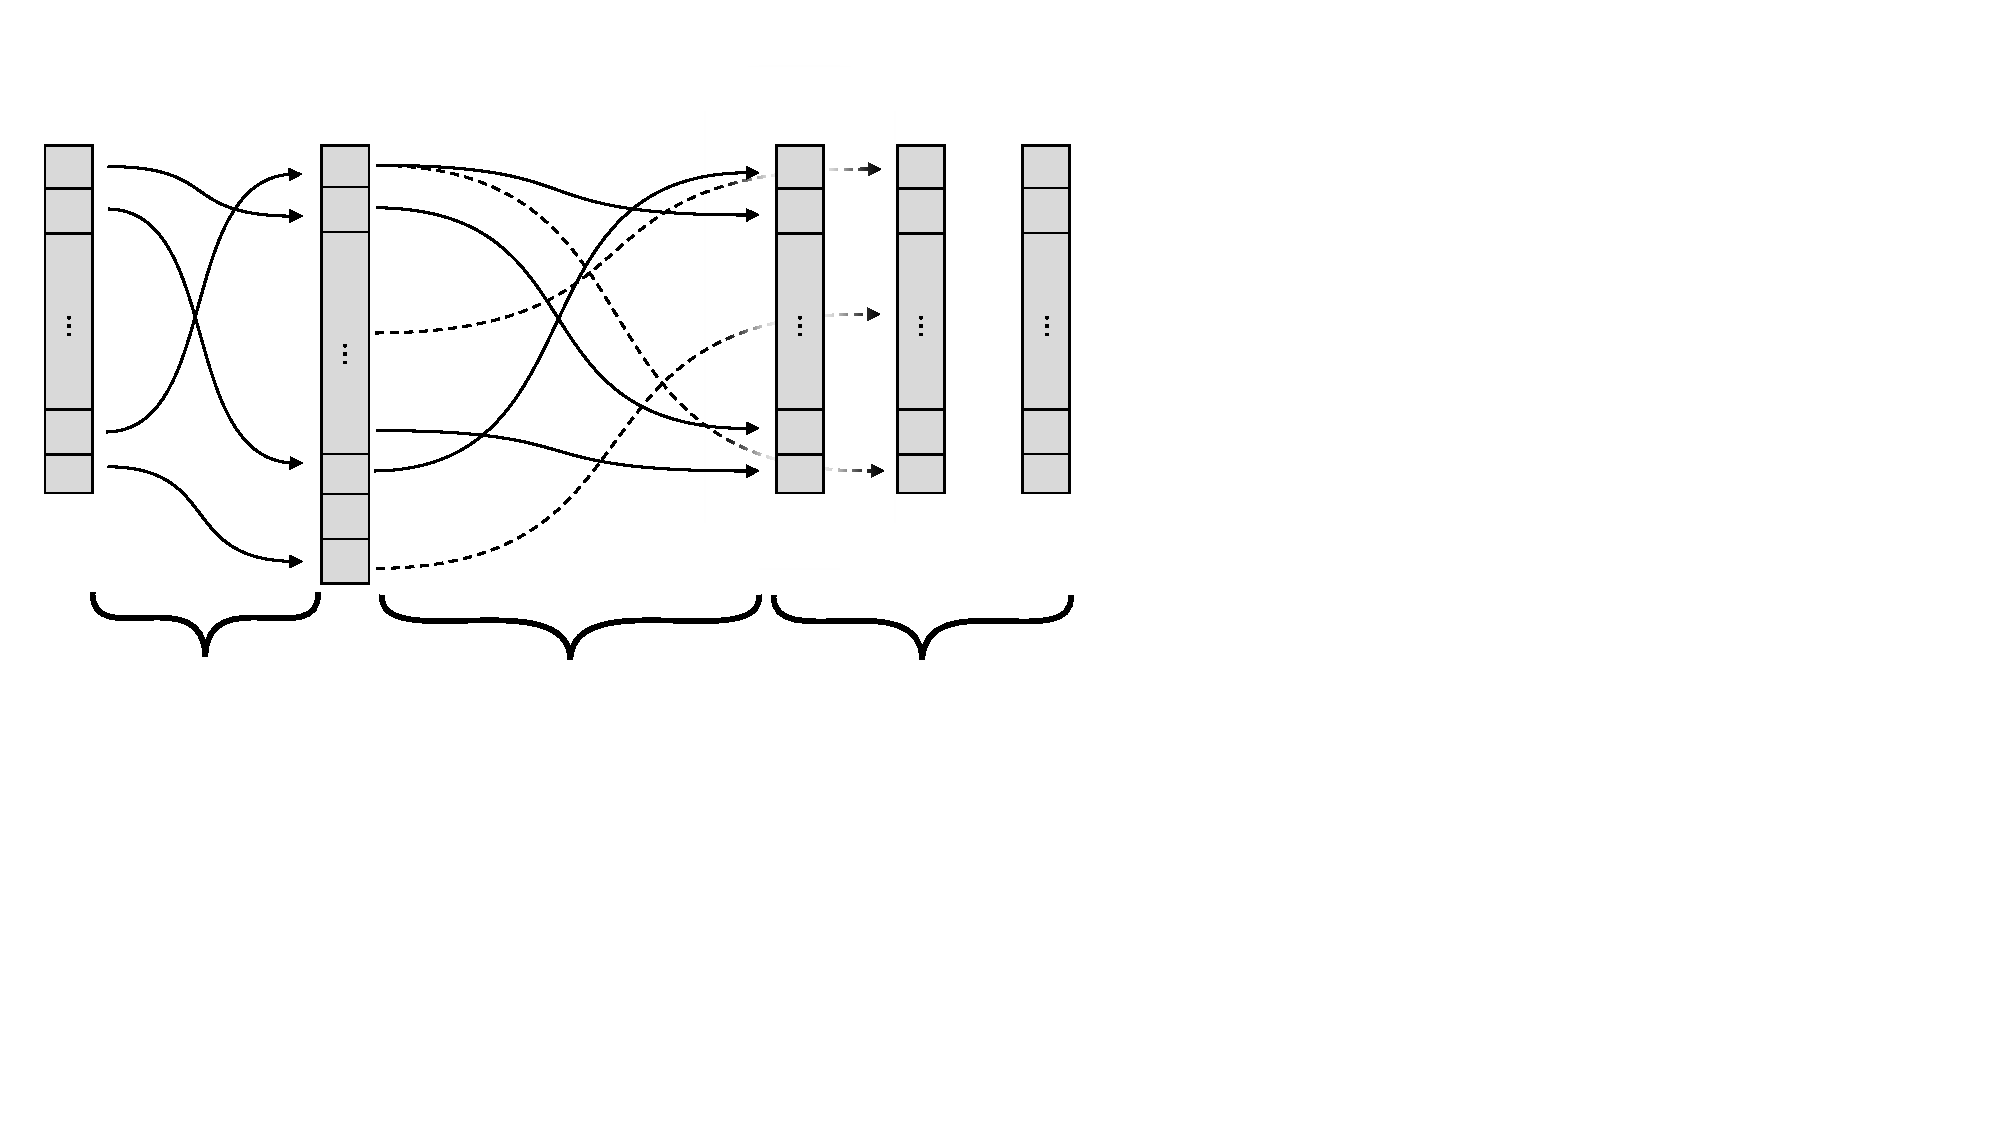
\includegraphics[trim={0cm 7cm 14cm 1cm},clip,width=\textwidth]{diga.pdf}}};
		\draw (-7.9cm,4cm) node {\large$Y$};
		\draw (7.2cm,4cm) node {\large$X$};
		\draw (-3.7cm,4cm) node {\large$\hat Y$};
		%	\draw (3.8cm,4.6cm) node {\large Selections w/ $h_0(x),h_1(x)$};
		\draw (3.3cm,4cm) node { \large$Y'_0$};
		\draw (5.2cm,4cm) node { \large$Y'_1$};
		
		\draw (-5.8cm,-4.5cm) node { Cuckoo hash w/ };
		\draw (-5.8cm,-5.0cm) node { $\textsc{encode}(Y)$ \& oblv. };
		\draw (-5.8cm,-5.5cm) node { permutation};
		
		
		\draw (-0.3cm,-4.5cm) node { Select Cuckoo locations w/ };
		\draw (-0.3cm,-5.0cm) node {  $\textsc{encode}(X)$ \& Oblv.};
		\draw (-0.3cm,-5.5cm) node { switching net.};
		
		
		
		\draw (5.2cm,-4.5cm) node { Compare w/ circuit };
		\end{tikzpicture}}
	\caption{Overview of the join protocol using oblivious switching network.}
\end{figure}
\fi
\subsection{Randomized Encodings}

Randomized encodings enable the parties to coordinator their secret shares without revealing the underlying values. Crucially, the equality  of two randomized encodings implies the equality of the encoded value but nothing more. The ideal functionality of the encoding process is given in \figureref{fig:randomized-encode-ideal}. It considers two commands which allow the parties to initialize the internally stored key $k$ and later generate encoding under that key. In particular, the parties are allowed to send secret shares of a value $x$  to the ideal functionality and destinate which party should learn the encoding. 
\iffullversion
 We define this idea functionality to allow a modular design and facilitate future improvements should a more efficient implementation be described. This functionality has several interesting properties. First, all encoding that have not been observed are uniformly distributed in that parties view. Secondly, learning an encoding $F_k(x)$ does not reveal any information about $x$ beyond being able to compare it for equality with other encodings.
\fi

\begin{figure}[ht]
	\framebox{\begin{minipage}{0.95\linewidth}
			Parameters: $N$ parties denoted as party 0 through party N-1. The input domain $\{0,1\}^\sigma$ and output domain $\{0,1\}^\ell$ for a pseudorandom function $F$.
			
			\begin{enumerate}
				\item[] [Key Gen] Upon receiving command $(\textsc{KeyGen})$ from all parties, sample a uniformly random key $k$ from the key space of $F$ and store it internally.
				
				\item[] [Encode] Upon receiving command $(\textsc{Encode}, \share x, i)$ from all parties, if $k$ is uninitialized compute $F_k(x)$ and send it to party $i$. 
			\end{enumerate}
	\end{minipage}}
	\caption{The Randomized Encoding ideal functionality \f{encode}}
	\label{fig:randomized-encode-ideal}	
\end{figure}


\paragraph{LowMC Encodings.}
We realize this functionality using the LowMC circuit\cite{lowmc} which computes a pseudorandom permutation. When implemented with the honest majority MPC protocols\cite{aby3, highthroughput}, this approach results in extremely high throughput. For instance, our implementation can compute one million encodings in one second.

LowMC is a family of MPC optimized block ciphers based on a binary substitution-permutation network. The cipher is parameterized by a block size $n$, keys size $\kappa$, s-boxes per layer $m$ and the desired data complexity $d$. 
\iffullversion
Given the desired security level, e.g. 128 bits, the required number of rounds $r$ can then be computed as a function of these parameters. The structure of the cipher is specifically optimized to reduced the number of s-boxes (\textsc{and} gate) and the number of rounds. For each of the $r$ rounds, the cipher adds part of the key to the current state, multiplies it with a public binary matrix and then applies 3 bit s-boxes in parallel to a subset of the state. 
\fi
With respect to performance metrics, the most costly operation is the application of the s-boxes and the number of rounds required. 

An important observation of our protocol is that the adversary only sees a bounded amount of block cipher output. In particular, the number of blocks observed $d$ is exactly the size of the table which is being encoded. For our implementation we set $d=2^{30}$ and optimize the remaining parameters. Our second observation is that our protocol uses the cipher as a PRF and does not require a excessive number of output bits. The remaining parameters $n,m$ were optimized empirically and set to be $n=80$ and $m=14$ which resulting in $r=13$, unless otherwise stated. This results in the evaluation of the LowMC requiring 13 rounds of communication and a total of 546 \textsc{and} gates (bits of communication) to achieve a security level of $\kappa=128$ bits.


\subsection{Oblivious Switching Network}

A switching network was introduced by Mohassel and Sadeghian\cite{MS13} as a circuit that can obliviously transform a vector $A=\{A_1,...,A_n\}$ such that the output is $A'=\{A_{\pi(1)}, ..., A_{\pi(m)}\}$ for an arbitrary function $\pi : [m]\rightarrow[n]$. The protocol of \cite{MS13} was designed in the two party setting where the first party inputs $A$ while the second party inputs a description of $\pi$. \iffullversion
This switching network require  $O(n\log n)$ cryptographic operations. Building on this general paradigm, we 
\else 
We
\fi
introduce a new oblivious switching network protocol tailored for the honest majority setting which significantly improves the efficiency. In particular, our protocol has linear overhead and is information theoretic secure. 

The ideal functionality of our protocol is given in \figureref{fig:perm-ideal} with three parties, a \emph{programer}, a \emph{sender} and a \emph{receiver}. The programmer has a description of  $\pi$ while the sender has a vector $A$ containing $n$ elements each consisting of $\sigma$ bits. The programmer and the receiver are output a 2-out-of-2 secret sharing of $A'=\{A_{\pi(1)}, ..., A_{\pi(m)}\}$.


The protocols and functionality described below assume the vector being transformed is the private input of the sender. However, our larger join protocols require the transformations to be applied to secret shared vectors. In particular, parties 0 and 1 both hold secret shares of $A$. This is achieved by using the oblivious switching protocol to transform the shares of the sender. The programmer who knows the program $\pi$ can then locally permute their local shares and combine this with the output of the oblivious switching protocol.

\begin{figure}[ht]
	\framebox{\begin{minipage}{0.95\linewidth}
			Parameters: $3$ parties denoted as the \emph{programmer}, \emph{sender} and \emph{receiver}. Elements are strings in $\{0,1\}^\sigma$. An input vector size of $n$ and output size of $m$.
			
			\begin{enumerate}
				\item[] [Switch] Upon the command $(\textsc{switch}, \pi)$ from the \emph{programmer} and $(\textsc{switch}, A)$ from the \emph{sender}, the functionality performs:
				\begin{enumerate}
					\item Interpret $\pi: [m]\rightarrow [n]$ as a function and $A\in \{0,1\}^{n\times \sigma}$ as a vector of $n$ elements. 
					\item Uniformly sample two $m$ elements vector $B^0, B^1\gets \{0,1\}^{m\times \sigma}$ s.t.  $\forall i\in [m], A_{\pi(i)} = B^0_i \oplus B^1_i$.
					\item Send $B^0$ to the \emph{programmer} and $B^1$ to the \emph{receiver}.
				\end{enumerate}
			\end{enumerate}
	\end{minipage}}
	\caption{The Oblivious Switching Network ideal functionality \f{switch}}
	\label{fig:perm-ideal}	
\end{figure}


\paragraph{Permutation Network}

We begin with a restricted class of switching networks where the programming function $\pi$ is injective. That is, each input element $A_i$ will be mapped to a maximum of one location in the output. 

The programmer samples two random functions $\pi_0,\pi_1$ such that $\pi_1 \circ \pi_0 = \pi$, $\pi_0$ is bijective and $\pi_1$ is injective. The programmer sends   $\pi_1$ to the receiver and $\pi_0$ and a vector $S\gets \{0,1\}^{\sigma\times n}$ to the sender who sends $T := \{A_{\pi(1)} \oplus S_0, ...,A_{\pi(n)} \oplus S_n \}$. The final shares of the permuted $V$ are defined as the programmer holding $\{S_{\pi_1(1)}, ..., S_{\pi_1(m)}\}$ and the receiver holding $\{T_{\pi_1(1)}, ..., T_{\pi_1(m)}\}$.
\iffullversion

%LWZ11 = https://eprint.iacr.org/2011/429.pdf
The simulatability of this protocol is straight forward and follows a similar logic as the oblivious shuffle protocol of Laur et al.\cite{LWZ11}. 
The view of the sender contains a uniformly distributed permutation of $n$ elements $\pi_0$ and a uniformly distributed vector $S$. Similarly, the view of the receiver contains $\pi_1: [m]\rightarrow [n]$ which is uniformly distributed (when $\pi_0$ is unobserved) and the vector $T$ is uniformly distributed given that it is masked by $S$. 
\fi
One important observation of this protocol is that $\pi_0,S$ can be generated locally by parties 0 and 1 using a common source of randomness, e.g. a seeded PRG. This reduces the rounds to 1 and linear communication complexity. 

\paragraph{Universal Switching Network}\label{sec:switch}

A universal switching network with an \emph{arbitrary} program $\pi : [m]\rightarrow [n]$ can be constructed in three phases\cite{MS13}. In particular, the input vector $A$ will have three transformations applied $A\overset{\pi_1}{\rightarrow}B\overset{\pi_2}{\rightarrow}C\overset{\pi_3}{\rightarrow}D=\pi(A)$.
\begin{enumerate}
	\item $B:=\pi_1(A)$:  The input vector $A$ is permuted by the injective function $\pi_1:[m]\rightarrow[n]$ such that if $\pi$ maps an input position $i$ to $k$ outputs positions (i.e. $k=|preimage(\pi,i)|=|\{ j : \pi(j)=i \}|$), then there exists a $j$ such that $\pi_1(j)=i$  and $\{\pi_1(j)+ 1,...,\pi_1(j )+k \} \cap image(\pi) = \emptyset$. That is, wherever position $i$ is mapped by $\pi_1$, it should be followed by $k-1$ input that do not appear in the final output. The parties then use a permutation network to compute $B:=\pi_1(A)$.
	
	\item $C:=\pi_2(B)$: The intermediate vector $B$ is transformed by a duplication network $\pi_2:[m]\rightarrow[m]$ such that if position $A_i$ is mapped to $k$ positions in $\pi(A)$, then $\{ C_{j},...,C_{j+k}\} = \{A_i\}$ where $\pi_1(j)=i$. That is, $C$ takes $B$ and copies $B_{j}$ into the next $k-1$ positions. 
	
	\item $D:=\pi_3(C)$: The final transformation $\pi_3:[m]\rightarrow[m]$  permutes $C$ to have the same ordering as $\pi(A)$. That is, the elements $\{ C_{j},...,C_{j+k}\}$ which all have the value  $A_i$ are arbitrary mapped to the $k$ positions $\{ j : \pi(j)=i \}$.
\end{enumerate}
Observe that steps 1 and 3 can both be implemented using the oblivious permutation protocol.% However, note that our oblivious permutation functionality is defined for $m\leq n$ while the switching network has no such restriction. This can be overcome by artificially padding the input vector $V$ with dummy items to be of size $\max(m, n)$. 

The transformation by $\pi_2:[m]\rightarrow[m]$ can be characterized by a bit vector $b$ of length $m-1$ where the $i$th bit denotes whether the item at position $i$ should be copied into position $i+1$. This observation gives rise to a natural protocol: for $i\in [m-1]$, if $b_i=1$ then use MPC to copy $B_i$ into $B_{i+1}$. The primary challenge is to achieve this while using a constant number of communication rounds which prevents the use of a generic (secret sharing) MPC protocol such as \cite{aby3, highthroughput}.

To obliviously select $B_i$ or $B_{i+1}$ conditioned on the programming bit $b_i$ the output $C_{i+1}$ must be secret shared. The programmer knowns the bit $b_i$ while $B_i$ and $B_{i+1}$ are private input of the sender. The programmer and sender will output secret share $C^0_{i+1}, C_{i+1}^1$ of the value $C_{i+1}:=b_i B_i + (1-b_1)B_{i+1}$. The sender samples three random strings $C_{i+1}^1, w_0,w_1\gets \{0,1\}^\sigma$ and a random bit $\phi\gets \{0,1\}$. They construct two messages $m_0=B_{i+1}^1\oplus C_{i+1}^1\oplus w_\phi$ and $m_1= B_i\oplus C_{i+1}^1 \oplus w_{\phi\oplus 1}$. The sender sends $w_0,w_1$ to the receiver and sends $m_0,m_1,\phi$ to the programmer who sends $\rho=\phi\oplus b_i$ to the receiver. The final share are constructed by having the receiver send $w_\rho$ to the programmer who computes $C_{i+1}^0:=m_{b_i}\oplus w_{\rho}$.
\iffullversion

The simulation of this protocol has two key parts. First, party 0 learns only one of the keys $w_0,w_1$ which determines which of the secret share $(B_{i+1}\oplus C_{i+1}^1$ or $  B_i\oplus C_{i+1}^1)$ they can one-time-pad decrypt. As such, the other share is uniformly distributed in their view. Similarly, the bit $\rho$ that the programmer sends to the receiver is uniformly distributed given that $\phi$ is not contained in the view of the receiver. The remaining messages $w_0,w_1,\phi$ which are uniformly sampled are trivial to simulate. Moreover, sending these messages can be optimized away when a PRG seed is pre-share between the appropriate parties.
\else
Note that  $w_0,w_1,\phi$  are uniformly random and sending them can be optimized away when a PRG seed is pre-share between the appropriate parties.
\fi

The protocol just described considers the setting where the messages $B_i,B_{i+1}$ are the private input of the receiver. However, we require that at each iteration the messages being selected is either $C_i$ or $B_{i+1}$ where the former was computed in the previous iteration and is secret shared between the programmer and sender. Fortunately, a trivial modification yields the desired functionality. The sender inputs their share of $C_i$ instead if $B_i$ while the programmer computes $C_{i+1}^0:=m_{b_i}\oplus w_{\rho}\oplus b_iC_{i}^0$.  \figureref{fig:switching-net} provides a formal description of the full switching network protocol.

\begin{figure}[ht!]
	\framebox{\begin{minipage}{0.95\linewidth}\small
			Parameters: $3$ parties denoted as \emph{programmer}, \emph{sender} and \emph{receiver}. Elements are strings in $\{0,1\}^\sigma$. An input vector size of $n$ and output size of $m$.
			
			\begin{enumerate}[leftmargin=.2cm]
				\item[] [Permute] Upon the command $(\textsc{Permute}, \pi)$ from the \emph{programmer} and $(\textsc{Permute}, A)$ from the \emph{sender}.  $\pi: [m]\rightarrow [n]$ is parsed as a \emph{injective} function and  $A\in \{0,1\}^{n\times \sigma}$ as a vector of $n$ elements. Then:
				\begin{enumerate}[leftmargin=.8cm]
					\item The \emph{programmer} samples a uniformly random bijective function $\pi_0 : [n]\rightarrow[n]$ and computes the injective function $\pi_1 :[n] \rightarrow[m]$ such that $\pi_1\circ \pi_0 = \pi$.  $\pi_0 $ and a random vector $S\gets \{0,1\}^{n\times \sigma}$ are sent to the \emph{sender}.
					\item The \emph{sender} computes and sends $B := \{ A_{\pi_0(1)} \oplus S_1, ..., A_{\pi_0(n)} \oplus S_n\}$ to the \emph{receiver}.
					\item The \emph{programmer} sends $\pi_1$ and a random vector $T\gets\{0,1\}^{m\times\sigma}$ to the \emph{receiver} who outputs $C^0:=\{B_{\pi_1(1)} \oplus T_1,...,B_{\pi_1(m)}\oplus T_m\}$. The \emph{programmer} outputs $C^1:=\{ S_{\pi_1(1)}\oplus T_1,...,S_{\pi_1(m)}\oplus T_m\}$.
				\end{enumerate}
				
				\item[] [Switch] Upon the command $(\textsc{Switch}, \pi)$ from the \emph{programmer} and $(\textsc{Switch}, A)$ from the \emph{sender}. $\pi: [m]\rightarrow [n]$ is parsed as a function and  $A\in \{0,1\}^{n\times \sigma}$ as a vector of $n$ elements. Then:
				\begin{enumerate}[leftmargin=.8cm]
					\item If $n<m$, the \emph{sender} redefines $A$ to be $A := A || \{0\}^{(m-n)\times \sigma}$ and all parties redefine $n:=m$.
					\item The \emph{programmer} samples an injective function $\pi_1:[m]\rightarrow [n]$ such that for $i\in image(\pi)$ and $k=|preimage(\pi, i)|$, there exists a $j$ where $\pi_1(j)=i$ and $\{\pi_1(j+1), ...,\pi_1(j+k) \}\cap image(\pi)=\emptyset$.
					
					The \emph{programmer}  sends $(\textsc{Permute}, \pi_1)$ to \proto{switch} and the \emph{sender} sends $(\textsc{Permute}, A)$. The \emph{programmer} receives $B^{0}\in \{0,1\}^{m\times \sigma}$ in response and the \emph{receiver} receives $B^{1}\in \{0,1\}^{m\times \sigma}$. 
					
					\item The \emph{programmer}  computes the vector $b\in\{0,1\}^{m}$ such that for $i\in image(\pi)$ and $k=|preimage(\pi, i)|$, $b_j = 0$ and $b_{j+1}=...=b_{j+k}=1$ where $\pi_1(j)=i$.
					
					The \emph{receiver} samples three $m$ element vectors $C^{1}, W^0,W^1\gets \{0,1\}^{m\times \sigma}$ and $\phi\gets\{0,1\}^m$. They set $C^{1}_1:=B^{1}_1$ and computes 
					\begin{align*}
						M^0_i&:= B^1_{i}\ \ \, \oplus C^{1}_i \oplus W^{\phi_i}_i\\
						M^1_i&:= C^1_{i-1} \oplus C^{1}_i \oplus W^{\phi_i\oplus 1}_i
					\end{align*}
					for $i\in \{2,...,m\}$. The \emph{receiver} sends $M,\phi$ to the \emph{programmer} and $C^{1},W$ to the \emph{sender}. The \emph{programmer} sends $\rho:=\phi\oplus b$ to the \emph{sender} who responds with $\{ W^{\rho_i}_i : i\in [m] \}$. The \emph{programmer} defines $C^{0}_1:=B^{0}_1$ and computes 
					$$
						C^{0}_i:= M^{b_i}_i \oplus W^{\rho_i}_i\oplus b_iC^{0}_{i-1}
					$$
					for $i\in \{2,...,m\}$.
					\item The \emph{programmer} computes the permutation $\pi_3$ such that for  $i\in image(\pi)$ and $k=|preimage(\pi, i)|$, $\{\pi_3(\ell) : \ell\in preimage(\pi, i)\}=\{j, ..., j +k\}$ where $i=\pi_1(j)$.	The \emph{programmer} sends $(\textsc{Permute}, \pi_3)$ to \proto{switch} and the \emph{sender} sends $(\textsc{Permute}, C^{1})$.  The \emph{programmer} receives $S\in \{0,1\}^{m\times \sigma }$ in response. The \emph{receiver} receives and outputs $D^{1}\in \{0,1\}^{m\times \sigma }$.
					
					The \emph{programmer} outputs $D^{0}_i:=S_i\oplus C^{0}_{\pi_3(i)}$ for $i\in [m]$.
				\end{enumerate}
			\end{enumerate}
	\end{minipage}}
	\caption{The Oblivious Switching Network protocol \proto{switch}. }
	\label{fig:switching-net}	
\end{figure}

\iffullversion
\paragraph{Arithmetic Shares}

The presentation above is framed in terms of binary secret shares. However, the same protocol strategy can work equally well for arithmetic shares. The main modification is that XOR operations in $\mathbb{F}_{2^\sigma}$ need to be appropriately replaced with addition and subtraction operations in $\mathbb{Z}_{2^\sigma}$. 
\fi

\subsection{Join Protocols}\label{sec:join}

Our join protocol can be divided into four phases:

\begin{enumerate}
	\item Compute randomized encodings of the joined on columns/keys. 
	\item Party 1 constructs a cuckoo table for table $Y$ and arranges the secret shares using an oblivious permutation protocol. 
	\item For each row $x$ in $X$, party 0 uses an oblivious switching network to map  the corresponding location $i_1,i_2$ of the cuckoo hash table to a secret shared tuple $(x, y_{i_1}, y_{i_2})$.
	\item The joined on column(s) of $x$ is then compared to that of $y_{i_1}, y_{i_2}$. If there is a match the output values are constructed. Otherwise the output row is set to \texttt{NULL}.
\end{enumerate} 

\paragraph{Randomized Encodings}
We begin by generating randomized encodings of the columns being joined on. For example, 
\iffullversion
$$
	\texttt{select }* \texttt{ from } X \texttt{ inner join } Y \texttt{ on } X_1 = Y_1 \texttt{ and } X_2 = Y_3
$$

\else
selecting all columns of $X$ and $Y$ where $X_1 = Y_1 \texttt{ and } X_2 = Y_3$.
\fi
In this case there are two joined on keys, $X_1,X_2$ from $X$ and $Y_1,Y_3$ from $Y$. Our protocol requires that the parties generate a randomized encoding for each row of $X$ and $Y$. That is, for all $i$ the parties must send a secret share of $\share{X_1[i] || X_2[i]}$ and $\share{Y_1[i] || Y_3[i]}$ to \f{encode} where $||$ denotes concatenation. In general, there can be an arbitrary number of joined on keys. 

There are two major challenges to efficiently implement this functionality in a composable setting. First, the encoding functionality takes as input a secret shared value consisting of $\sigma$ bits. However, the number of bits being encoded is a function of the joined on columns. To support this, we present a procedure to reduce the size of the joined on keys. 

Specifically, once the tables being joins on have been specified, the parties jointly pick a random matrix $E\gets\{0,1\}^{m\times \sigma}$ where $m$ denotes the total bit length of the columns being joined on. The parties can then locally multiply the concatenated keys with $E$, e.g. $\share{E_x}=\share{X_1[i] || X_2[i]} E$ and $\share{E_y}=\share{Y_1[i] || Y_3[i]} E$. These secret shares are then be forwarded to the \f{encode}.

To preserve security we require the probability of the following game outputting 1 be negligible in $\lambda$. 
\begin{quote}
Have the adversary select two sets $X,Y\subset \{0,1\}^{m}$ of size $n_1,n_2\in poly(\lambda)$  respectively and then a uniformly random matrix $E\gets \{0,1\}^{m\times \sigma}$ is sampled. If there exists distinct $x\in X$ and $y\in Y$ such that $xE = yE$, output 1, otherwise 0. 
\end{quote}

First observe that this use of $E$ is a universal hash function. Therefore, fixing any $x\in X, y\in Y$, it holds that $\Pr[xE=yE]=2^{-\sigma}$. Following the same logic as the hash to smaller domain technique of \cite{usenix:PSZ14,CLR17}, the overall probability of a collision is $2^{-\sigma}n_1n_2$ which results in a statistical security parameter of $\sigma -\log_2(n_1)-\log_2(n_2)$. We ensure that this value is equal to the target statistical  security parameter $\lambda$.
\iffullversion
 In practice, we set $\lambda=40$ and choose $\sigma =80$ if $n_1=n_2=n\leq 2^{20}$ and $\sigma=100$ otherwise (supporting $n\leq 2^{30}$). 
\fi

%\todo{Show that this holds and that $\sigma=80$ is chill for $\lambda = 40$.}

A second issues is that after a previous join operation, some (or all) of the rows being joined can be invalid with duplicate keys. We require that the randomized encodings of these keys not reveal which rows are invalid. This is achieved by secret sharing a bit for each row that encodes whether the row is valid. Given this bit \share{b}, the parties can generate a random $\sigma$ bit share $\share{r}$ for each value $\share{x}$ that is encoded. Before $\share{xE}$ is sent to \f{encode}, the parties compute $\share{x'}:=\share{xE}\oplus \share{\overline{b}}\share{r}$ and send $\share{x'}$ instead.
\iffullversion
 In the event that the current row is valid, this alteration has no effect on the computation due to \share{\overline{b}}\share{r} being a secret sharing of zero. However, when the row was invalid the value of $x'$ is uniformly distributed. 
\fi
 Following the same logic as before, the probability that $x'$ collides with some $y'$ is statistically negligible and therefore the resulting encoding is uniformly distributed and unique with overwhelming probability. 

%\todo{Pr. of collision.}

Putting everything together, the parties sample $E\gets\{0,1\}^{m\times \sigma}$ if $m>\sigma$ and $E=I$ otherwise. For each set of join on columns $\share{Z_{i_1}},...\share{Z_{i_l}}$ that are to be encoded, a secret shared value  $r\gets\{0,1\}^\sigma$ is sampled and the parties compute $\share{z'}:=\share{Z_{i_1}||...||Z_{i_l}}E \oplus \share{\overline{b}}\share{r}$. \share{z'} is sent to \f{encode}. Party 0 receives the randomized encodings $\mathbb{E}_x$ for the joined on keys of $X$ and party 1 receives the encodings $\mathbb{E}_y$ for $Y$.

\paragraph{Constructing the Cuckoo Table}

The next phase of the protocol is for party 1 to construct a secret shared cuckoo table for $Y$ where each row is inserted based on its encoding $\mathbb{E}_y$. Party 1 locally inserts the encodings $\mathbb{E}_y$ into a plain cuckoo hash table $T$ with $m$ slots using the algorithm specified in \sectionref{sec:prelim}. Party 1 samples an injective function $\pi : m\rightarrow m$ such that for the $i$th $e\in \mathbb{E}_y$ and $T[j]=e$, then $\pi(j)=i$.
\iffullversion
 That is, $\pi$ defines the mapping from each row's original position in the table $Y$ to the corresponding position in the cuckoo table $T$.
\fi

Recall that parties 0 and 1 respectively hold a 2-out-of-2 secret sharing $Y^0,Y^1$ such that $Y=Y^0\oplus Y^1$. 
Party 1 sends $(\textsc{Switch}, \pi)$ to \f{switch} and party 0 sends $(\textsc{Swich}, Y^0)$\footnote{Note that $Y^0$ has $n$ rows while $\pi$ is defined with an input vector containing $m\approx 1.6n$ rows. Party 0 will pad $Y^0$ with $m-n$ rows which contain all zeros. These will be mapped to the empty slots of the cuckoo table by the permutation/switching network.}. In response \f{switch} sends $\hat Y^{0,1}$ to party 1  and $\hat Y^{0,0}$ to party 2. Party 1 defines their output of this phase as $\hat Y^0:=\hat Y^{0,1} \oplus \pi(Y^1)$ and party 2 defines their output as $\hat Y^{1} =\hat Y^{0,0}$.
It is now the case that $\hat Y = \hat Y^0\oplus \hat Y^1$ is a valid secret shared cuckoo hash table of the original table $Y$.
\iffullversion
 In particular, for a given row $Y[i]$ with encoding $e=\mathbb{E}_y[i]$, there exists a $j\in \{h_1(e),h_2(e)\}$ such that  $\hat Y[j] = Y[i]$. Here, the $h_0,h_1$ functions are hash functions used to construct the cuckoo table $T$. Another important observation is that $\pi$ is a permutation and therefore the more efficient permutation protocol can be used in place of the universal switching protocol.

We note that some of the columns of the tables may be secret shared in arithmetic group as opposed to binary shares. In this case the switching network will use the appropriate arithmetic operation as note in \sectionref{sec:switch}. 
\fi

\paragraph{Selecting from the Cuckoo Table}

The next phase of the protocol is for each row of $X$, select the appropriate rows of $\hat Y$ so the keys can be compared. Party 0 knows that if the joined on keys of the $i$th row $X[i]$ will match with a row from $Y$, then this row will be at $\hat Y[j]$ for some $j\in \{h_1(e),h_2(e)\}$ where  $e=\mathbb{E}_x[i]$. 

To obliviously compare these rows, party 0 will construct two switching networks with programming $\pi_1,\pi_2 : n\rightarrow m$ such that if $h_l(\mathbb{E}_x[i])=j$ then $\pi_l(i)=j$. Each of these will be used to construct the tables $\share{\widetilde{Y}^1},\share{\widetilde{Y}^2}$ which are the result of applying the switching networks $\pi_1,\pi_2$ to $\share{\hat Y}$. 
\iffullversion
In particular, for the $i$th row $X[i]$ it is now the case that if $X[i]$ has a matching row in $Y$ then it will be contained at  $\widetilde{Y}^1[i]$ or $\widetilde{Y}^2[i]$. 
\fi


\paragraph{Inner Join}

Given the three secret shared tables $\share{X},\share{\widetilde{Y}^1},\share{\widetilde{Y}^2}$ as described above, the parties do a linear pass over the $n$ rows to construct the join between $X$ and $Y$. Recall that the inner join consists of all the selected columns from the rows $X[i],Y[j]$ where  the joined on keys of the rows $X[i]$ and $Y[j]$ are equal. Alternatively, an inner join can be thought of as the intersection between the joined on keys of $X$ and $Y$. 

If row $X[i]$ has a matching row in $Y$ then this row will occupy at most one of the rows ${\widetilde{Y}^1}[i],{\widetilde{Y}^2}[i]$. To determine which, the parties input the secret shared of these rows to an MPC protocol where the join on columns are compared. For each $i$ and rows ${\widetilde{Y}^1}[i],{\widetilde{Y}^2}[i]$ the bits $b_1[i],b_2[i]$ are generated where $b_l[i]=1$ iff the joined on columns if ${\widetilde{Y}^l}[i]$ are equal to that of $X[i]$. The MPC circuit then computes $b[i]=b_1[i]\oplus b_2[i]$ and $Y'[i]=b_1[i]{\widetilde{Y}^1}[i]\oplus b_2[i]{\widetilde{Y}^2}[i]$. $b[i]$ encodes whether the $i$th row of the output table is valid. If it is valid, then $Y'[i]$ is the row of $Y$ which matches $X[i]$.

Next, the \texttt{where} clause of the query and any addition computation which is specified by the \texttt{select} clause is computed. The \texttt{where} clause further filters the output table as a function of $Y'[i]$ and $X[i]$. 
\iffullversion
For example, the query may specify that only rows where $Y_2'[i] + X_3[i] > 22$  are to be selected. Regardless of the exact where clause, the 
\else 
The
\fi
MPC protocol updates the valid bit as $b[i] := b[i] \wedge P(Y'[i], X[i])$ where $P: \mathcal{Y}\times \mathcal{X} \rightarrow \{0,1\}$ is the predicate function specified by the \texttt{where} clause.

Finally, the additional computation specified by the \texttt{select} query is performed. Specifically, the columns of the output table can either be directly copied from the input tables $X,Y$ or can be a function of the given row. 
\iffullversion
For example, the query could be of the form 
$$
\texttt{select } X_1, Y_2 + X_3 \texttt{ from } X \texttt{ inner join } Y \texttt{ on } X_1 = Y_1
$$
In this case the first column of the output will be $X_1$ while the second column will consist of the second column of $Y$ plus the third column of $X$. 
\fi
In general we view the \texttt{select} clause as a function which takes the two rows $X[i]$ and $Y'[i]$ and computes a new row with the specified columns. 

\iffullversion
Several optimizations can be applied to this protocol. First, observe that only columns of $Y$ which explicitly appear in the query need to be input to the switching networks. This reduces the amount of data to be sent and improves performance. Secondly, when comparing the joined on columns, instead of computing the equality circuit between all of these columns it suffices to compare the randomized encodings. In the event that the joined on column(s) contain many bits, comparing the encodings can reduce the size of the equality circuit. In addition, observe that including columns from $X$ in the output table is essentially free due to these secret share columns simply being copied from $X$. Leveraging this the queries can be optimized by ensuring that the majority of the output columns are taken from $X$. Moreover, if a joined on column from $Y$ is in the \texttt{select} clause, this output column can be replaced with the matching column in $X$.

Also observe that the computation perform heavily lends itself to SIMD instructions. That is, the same computation is repeatedly applied to each row of the output table. Modern MPC protocol such as the ABY$^3$ framework \cite{aby3,highthroughput} are optimized for this setting and can process billions of binary circuit gates per second\cite{highthroughput}. In addition the ABY$^3$ framework can switch between using binary and arithmetic circuits based on which is most efficient for the given computation. 
\fi

\paragraph{Left/Right Join}

A left join query is similar to an inner join except that all of the rows from the left table $X$ are included in the output. In this case all of the output fields that are a function of the right table but do not have a matching row from the right table are initialized as a default value, typically \texttt{NULL}.  This type of join has the property that all of the output rows maintain their validity\footnote{More specifically, the output rows copy the validity bit $b[i]$ from the $X$ table.} and the valid bits $b[i]$ need not be updated. Instead the bits $b[i]$ as computed in the inner join are used to determine if the fields that are a function of $Y$ need to be initialized to the default value. That is, all rows that are in the inner join are computed as before and the remaining rows from $X$ use the bit $b[i]$ to initialize the missing values to the default. A right join can be implemented symmetrically.

\paragraph{Union and Set Minus}

Our framework is also capable of computing the union of two table. Specifically, we define the union operator as taking all of the rows from the left table and all of the rows from the right table that would not be present in the inner join. Note that the union operator assumes that the schemes of the two tables are identical. Somewhat surprisingly the protocol implementing union is conceptually similar to the inner join. The key observation is that the inner join computes a valid bit for each row of $X$ which encodes whether that row is in the intersection. By flipping this bit\footnote{Note that the special case where a row of $X$ is not valid as opposed to being outside the intersection must be handled.}, it now encodes whether that row is in $X\backslash Y$. Given such an operator the union of $X$ and $Y$ can trivially be constructed as $(X\backslash Y) || Y$ where the $||$ operator denotes the row-wise concatenation of $Y$ to the end of $X\backslash Y$.


\paragraph{Full Join}

A full join can be viewed as a hybrid between an inner join and a union. Specifically, the output table contains the inner of $X$ and $Y$ which is then unioned with $X$ and $Y$ on the right side. Put another way, a full join consists of the inner join where the missing rows from $X,Y$ additionally included. 

In the general case we construct a full join protocol using two other join operations. First a left join between $X$ and $Y$ is performed. As a result the rows in the inner join are correctly computed and all records from $X$ are contained in the output table. What remains is to add all of the missing rows from $Y$ which is achieved by taking the union with the output table and $Y$. The overhead of this protocol is effectually twice that of the other protocol.

We note that under some restrictions on the tables being joined, a more efficient protocol for full joins can be achieved. We defer an explanation of this technique to \sectionref{sec:threatlog}.

%
%
%Next, we introduce a second protocol that requires $X$ and $Y$ to contain only valid rows.
%This join is implemented in two phases. First the union of just the joined on columns is performed, denoted as $Z=X\cup Y$. The parties will then generate randomized encodings for $Z,X,Y$. The encodings for $Z$ will be revealed to all parties while $X,Y$ are respectively revealed to party 0,1. Importantly, before these encoding are generated, the rows of the $Z$ table must be obliviously shuffled. This ensure that ordering information between $Z$ and $X,Y$ does not leak information. 
%
%Given these encodings, party 0 can use an oblivious permutation to reorder the rows of $X$ such that the encodings of $X$ and $Z$ are aligned. Similarly, party 1 can perform the same operation for $Y$. Let these new tables be denoted as $X',Y'$ respectively. In particular, the encodings for row $X'[i]$ should The final full join table $Z'$ can then be constructed by applying the select and where clause to each concatenated row $X'[i] || Y'[i]$.
%
%Several optimizations can be applied to this strategy. First, the $Z$ tables is computed the joined on columns of $X,Y$ can be compressed to a maximum of $\sigma$ bits by multiplying them with a random linear matrix as was performed in \sectionref{sec:join}. As a result, less data needs to be joined on in the union protocol resulting in improved performance. When the encodings for $X,Y$ are later computed, these compressed values can be reused. Secondly, in the case that there are several tables $U,...,X,Y$ all being full joined, the protocol can achieve even better performance. First, the union of the joined on columns of these tables is computed as before. Let this table be denoted as $Z$.  The original
%
%


%\subsection{Cardinality Revealing Joins}
%
%In some situations it may be possible to allow the cardinality of the join to be revealed to the parties. This is turn can be leveraged in conjunction with the uniqueness property of the joined on columns to improve the efficiency of the protocols.  Consider computing the inner join with an intersection size of $n'$. This immediately implies that the parties know $n-n'$ of the output table are invalid rows. However, which rows these are can convey significant information about the data that is contain. Say table $X$ is joined with $A,B,C,D,...$ and for all of these joins the first row of $X$ is always in the inner join. All of the parties now know that the first row of $X$ is contained in each of these other tables. For example, consider the $X$ being hospital patients, $A$ containing the last admission date and $B$ containing a list of patients with HIV/AIDS. When combined with other information, learning that the first row of $X$ was admitted on some day $A[j]$ and has HIV/AIDS could potentially reveal who this person is. 
%
%To prevent the parties correlating information in this way we introduce a new set of join protocols specifically designed for this setting. The core technique is for party 0 and 1 to sample random permutation networks for each table. After all permutations are applied, the row order of both tables are uniformly distributed in the view of the parties. The randomized encoding phase can then be performed where party 0 learns the encodings for $X$ and party 1 learns them for $Y$. Instead of proceeding with the construction of the cuckoo table, the parties can directly exchange the encodings. This immediately reveals which rows are in the intersection and allows the parties to construct the output table from the randomized $X,Y$ tables by directly copying the appropriate secret shares. This technique can be extended to the other types of joins listed above. In all cases the knowledge of the randomized encodings allow the parties to appropriately construct the output table. We note that this approach is similar to \cite{LTW13}
%

\subsection{Non-unique Join on Column}


When the uniqueness of the columns being joined on does not hold the security guarantees begin to erode. Recall that the randomized encodings for $X,Y$ are revealed to party 0,1 respectively and therefore some of these encodings will be duplicates due to the joined on columns not containing unique values. Learning the distribution of these duplicates reveals that the underlaying table has the same distribution. In the event that only one of the tables contains duplicates, the core protocol can naturally be extended to compute the various join operations subject to party 0 learning the duplicate distribution. This is achieved be requiring the left table $X$ contain the duplicates rows. After learning the randomized encodings for this table party 0 can program the switching networks appropriately to query the duplicate locations in the cuckoo hash table. 


When both tables contain duplicates we fall back to a less secure protocol architecture. First, party 1 samples two random permutations $\pi_0,\pi_1$ and computes $X'=\pi_1(X),Y'\pi_2(Y)$ using the oblivious permutation protocol. Party 0 then learns all of the randomized encodings for the permuted tables $X'$ and $Y'$. Given this, party 0 can compute the size of the output table and informs the other two parties of it. Alternatively, an upper bound on the output table size can be communicated. Let $n'$ denote this value. Party 0 can then construct two switching networks which maps the rows of $X'$ and $Y'$ to the appropriate rows of the output table. The main disadvantage of this approach is that party 0 learns the size of the output, the distribution of duplicate rows and how these duplicate rows are multiplied together. However, unlike \cite{LTW13} which takes a conceptually similar approach, our protocol does not leak any information to parties 1 and 2, besides the value $n'$.

%When both tables contain duplicates we fall back to the less secure protocol architecture of Laur et al.\cite{LTW13}. In particular, this style of protocol  performs an oblivious shuffling of the table rows and then reveals all of the randomized encodings to all of the parties. Given this information the parties can construct the desired join. We suggest that the performance of these two primitive can be improved over \cite{LTW13} by 1) implementing the random shuffle using two random permutation networks from \sectionref{sec:switch} where party 0 and 1 both privately sample one of the permutations. 2) Replace the use of AES with our improved randomized encodings (LowMC and random binary matrix). Given these optimization the overhead of these protocols should be comparable to our standard join techniques. The major shortcoming of this approach is that the duplicate distribution and the size of join is revealed to all of the parties. As discussed in the related work section, this can limit several important application such as threat log comparison. 

\subsection{Revealing Results}

Revealing the values contained in a secret shared table in general requires two operations. First observe that the data in the invalid rows is not cleared out by the join protocols. As such naively reconstructing these rows would lead to significant leakage. Instead the bitwise \textsc{and} between the valid bit and the row is computed. This ensures that all invalid rows have a deterministic value and therefore can be simulated. The second operation is to perform an oblivious shuffle of the rows. This operation randomly reorders all the rows without revealing the ordering to any of the parties. The necessity of this operation stems from the  row ordering (prior to the shuffle) being input dependent. Moreover, this ordering can be used to correlate between two different output tables. In particular, the row ordering of say $X\cap Y$ and $X\cap Z$ will be the same up to some rows being valid while other may not. In the case of sets this ordering does not reveal additional information since it can be inferred given the ideal output, e.g. set intersection, then the shuffling can be omitted. However, this is not true in general when the items being joined are key-value pairs. 


\section{Computing a Function of a Table}\label{sec:card}

In addition to join queries, our framework can perform computation on a single secret shared table. For example, selecting $X_1+X_2$  where $X_3>42$. This type of select statement can easily be express with any generic MPC protocol, in particular \cite{aby3, highthroughput}. The key property is that all of the operations are with respect to a single row of $X$. As such, this computation can be expressed as a circuit and evaluated in parallel on each row. 

Our framework also considers a second class of functions on a table that allow computation between rows. For exampled, computing the sum of a column. We refer to this broad class of operations as an aggregation function. Depending on the exact computation, various levels of efficiencies can be achieved. Our primary approach is to employ the ABY$^3$ framework \cite{aby3} to express the desired computation in the most efficient way possible and then to evaluate the resulting circuit. Next we highlight a sampling of some important aggregation operations:
\begin{itemize}
	\item Sum: In this case there is a column of secret shared $\ell$-bit values that need to be added together.  The default secret sharing format that we employ is a binary sharing. First all $n$ values are converted to an arithmetic sharing which requires $n\ell$ binary gates \cite{aby3}. The parties can then locally sum the arithmetic shares without any additional communication. This approach requires $\ell$ rounds of communication. Alternatively, $n\ell\log \ell$ binary gates and $\log \ell$ rounds can be used\cite{aby3}. One important note is that each row must be check to ensure that it is valid. We propose doing this by computing the logical AND between the valid bit and the value being summed before it is converted to an arithmetic share. Given this, the correct result is the sum of the arithmetic shares, regardless of the validity of any given row.
	
	\item Count/Cardinality: Here, we consider two cases. 1) In the general case we also assume that the actual secret shared table containing the join is desired. Here, the count/cardinality can be computed in a similar way as sum except that the summation is directly over the valid bits. The more efficient bit injection protocol\cite{aby3} can be used to convert each bit to an arithmetic sharing in a constant number of rounds. In particular, the malicious secure bit injection protocol provided in \cite{aby3} is suggested due to it reducing the overall communication. 
	
	2) In the case that only the cardinality of a join is desired, a more efficient protocol can be applied. First, let us assume that only party 2 should learn the cardinality. Parties 0 and 1 generate the randomized encodings for the two sets as done in the standard join protocol. These encodings are then sent to party 2 in a random order. The cardinality of the intersection can then be securely computed by counting the encodings that appear in both sets. In the event that party 0 or 1 should also learn the cardinality, party 2 can send the final result to them. 
	
	\item  Min/Max: Unlike computing sums, logical operations such as max are most efficiently computed over using a binary sharing format. In particular, we propose a binary tree structure where elements are compared and the min/max item is propagated. Concerning invalid rows, these values can be initialized to the maximum or minimum value to guarantee that the other value will be propagated. The overall complexity of this approach is $O(n\ell)$ binary gates and $O(\ell log n)$ rounds when using a basic comparison circuit\cite{aby3}.
\end{itemize}

\section{Beyond Three Parties}


In some settings where many parties are providing tables to be computed on, the three party requirement with at most one corruption may not be adequate. In particular, a larger corruption threshold such as 3-out-of-5 or 4-out-of-7 may be desirable. Our protocol can naturally be extended to these setting with some caveats. First, the binary circuit based MPC protocol\cite{highthroughput}, which our standard three party protocol relies on, can be naturally extended to these larger (honest majority) corruption thresholds. Alternatively, several other suitable protocol such as\cite{DBLP:conf/crypto/ChidaGHIKLN18} have been proposed. This change immediately implies that no minority set of corrupted parties can decrypt/reconstruct the secret shared tables. However, our three party protocol also requires party 0 and 1 learning the randomized encodings in the clear.  As has previously been described, when the adversary learns both sets of randomized encodings they can infer information about the cardinality of the join. As such, our protocol offers two levels of security. When the adversary corrupts parties 0 and 1 the cardinality of the join is revealed. Otherwise, if an honest majority is present then the view of the corrupted parties can be simulated in the semi-honest setting. 



